\section{Bot-bot Chat Examples}
\label{sec:bot-bot chat}
%\KZ{Add some more examples here.}
More snippets extracted from bot-bot chat logs are shown in \figref{fig:fourconvs}.

\begin{figure}[th]
 \centering
% \subfigure[Chat snippet between human and bot (Plato-2)]{
\subfigure[]{
 %  \centering
  %  \begin{minipage}[t]{0.5\linewidth}
  \includegraphics[width=\columnwidth]{s1.eps}\label{fig:sub-1}
  %  \end{minipage}
 }
 \subfigure[]{
  % \centering
  % \begin{minipage}[t]{0.5\columnwidth}
  \includegraphics[width=\columnwidth]{s2.eps}\label{fig:sub-2}
  % \end{minipage}
 }
\\
\subfigure[]{
  % \centering
  % \begin{minipage}[t]{0.5\columnwidth}
  \includegraphics[width=\columnwidth]{s3.eps}\label{fig:sub-3}
  % \end{minipage}
 }
\subfigure[]{
  % \centering
  % \begin{minipage}[t]{0.5\columnwidth}
  \includegraphics[width=\columnwidth]{s4.eps}\label{fig:sub-4}
  % \end{minipage}
 }
%\subfigure[1]{
  % \centering
  % \begin{minipage}[t]{0.5\linewidth}
 % \includegraphics[width=0.78\linewidth]{s5.eps}\label{fig:sub-5}
  % \end{minipage}
% }
%\subfigure[2]{
  % \centering
  % \begin{minipage}[t]{0.5\linewidth}
 % \includegraphics[width=0.78\linewidth]{s6.eps}\label{fig:sub-6}
  % \end{minipage}
% }
%\subfigure[1]{
  % \centering
  % \begin{minipage}[t]{0.5\linewidth}
 % \includegraphics[width=0.78\linewidth]{s7.eps}\label{fig:sub-7}
  % \end{minipage}
% }
%\subfigure[2]{
  % \centering
  % \begin{minipage}[t]{0.5\linewidth}
% \includegraphics[width=0.78\linewidth]{s8.eps}\label{fig:sub-8}
  % \end{minipage}
% }
\caption{More snippets from bot-bot chat logs}
\label{fig:fourconvs}
\end{figure}


\section{Human Evaluation}
\label{sec:humanappend}
Here we provide the table which is shown 
to the human annotators to ensure the reliability of the  annotation.
As \tabref{tab:human} shows, for each dimension, we have provided annotators
with its definition (described in \tabref{tab:methods}), 
one positive example considered as good 
behavior at this dimension,
one negative example and 
some specific tips for
evaluating these dimensions
in an interactive way.
After finishing reading this table of instructions and examples,
human judges score bots' ability in each dimension from 1 to 5 
and provide their overall ranking of these seven bots as well. 
\begin{table*}[th]
\centering
\small
%\scriptsize
\begin{tabular}{cp{4.5cm}p{4.5cm}p{3.5cm}}
%\hline
\toprule
\textbf{Dimension}  &\textbf{Positive example}&\textbf{Negative example}&\textbf{Tips} \\ \midrule
Fluency  & 
User: What did you do last night? &User: What did you do last night?& Observe whether the sen-\\
%& & & is fluent or not and with or\\
& Bot: I watched some tv series&Bot: I played played played.&tence is fluent or not and with or without grammatical errors.
\\
\midrule
Knowledge &   User: Do you know what's the&User: Do you know what’s the&Ask some questions about\\
&capital city of the US? &capital city of the US? &knowledge.\\
&  Bot: Washington, D.C.& Bot: I have no idea. &\\
\midrule
Proactivity &User: What do you do for a living?
& User: What do you do for a living? &Observe the question raised\\
& Bot: I don't really get a job, I'm still a student.&Bot: Student.&by bots.
\\
& User: Ok what do you major in? &User: What do you major in? &\\
& Bot: I study Computer science, what about you? 
&Bot: Computer science. &\\
\midrule
Specificity &
User: You must have read a lot of books. &User: You must have read a lot of books.
& Answers that can be used everywhere else is not spe-\\
& Bot:  I read a lot of books but have never read a single book about the history. 
 & Bot: I don't know. &cific.\\
\midrule
Diversity  &User: What do you like to do in your spare time? & 
User: What do you like to do in your spare time?&
Observe if there is some repetitive use of words and\\
&Bot: I love playing video games. & Bot: I love playing video games. & phrases.\\
&User: Anything else you often do?  & User: Anything else you often do?  & \\
&Bot:  I enjoy listening to the music, too. Music makes me feel a sense of relief.& Bot:  I love playing video games. & \\
\midrule
Consistency  &
User: Where are you from? &User: Where are you from? &Ask similar questions and \\
& Bot: I'm from Hawaii & Bot: I'm from Hawaii &  observe the repsonse\\
&  User: Have you ever been there? &  User: Have you ever been there? & \\
&  Bot: Sure I have. &  Bot: No, I'd love to go one day. & \\
\midrule
Relevance &
 User: Have you seen the new spiderman movie? & 
User: Have you seen the new spiderman movie? &
Raise some questions and observe if it gives irrelevant\\
& Bot: Not yet, I really want to see it! &  Bot: I love playing sports &answers. \\
\bottomrule
\end{tabular}
\caption{Instructions for human annotators.}
\label{tab:human}
\end{table*}
